\section{Prospetto economico}
Vengono mostrati i prospetti economici per ciascuna fase di progetto, divisi per ruolo. Le fasi di \textbf{Analisi} e \textbf{Analisi di dettaglio} non sono a carico del committente.

\subsection{Analisi}
Nella fase di \textbf{Analisi} le ore sono suddivise nel modo seguente:
\begin{table}[H]
  \centering
  \begin{tabular}{|c|c|c|}
  \hline
  \textbf{Ruolo} &
  \textbf{Ore} &
  \textbf{Costo} \\
  \hline
  Responsabile & 35 & 1050\\
  \hline
  Amministratore & 27 & 540\\
  \hline
  Analista & 93 & 2325\\
  \hline
  Progettista & 0 & 0 \\
  \hline
  Programmatore & 0 & 0 \\
  \hline
  Verificatore & 41 & 615\\
  \hline
   \textbf{Totale} & \textbf{196} & \textbf{4530} \\
    \hline
  \end{tabular}
  \caption{Costo per ruolo, fase di Analisi}
\end{table}

I seguenti grafici mostrano visivamente come abbiano influiranno i ruoli per ore e costi nella fase di \textbf{Analisi}.
\begin{figure}[H]
\centering
\scalebox{0.6}{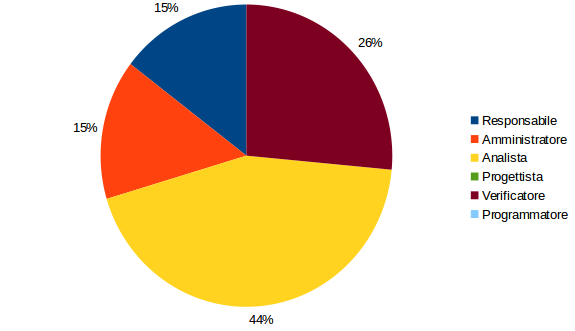
\includegraphics{img_peconomico/oreAnalisi.png}}
\caption{Ore per ruoli, fase di Analisi}
\end{figure}
\begin{figure}[H]
	\centering
	\scalebox{0.6}{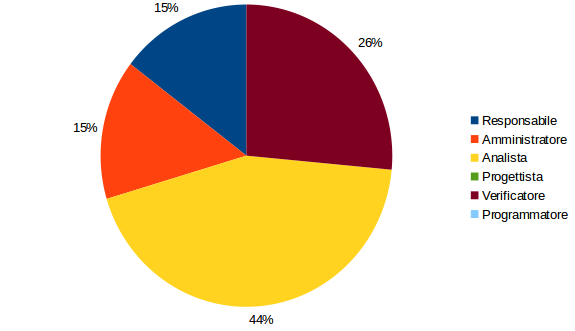
\includegraphics{img_peconomico/oreAnalisi.png}}
	\caption{Costi per ruolo, fase di Analisi}
\end{figure}

\subsection{Analisi di dettaglio}
Nella fase di \textbf{Analisi di dettaglio} le ore sono suddivise nel modo seguente:
\begin{table}[H]
	\centering
	\begin{tabular}{|c|c|c|}
		\hline
		\textbf{Ruolo} &
		\textbf{Ore} &
		\textbf{Costo} \\
		\hline
		Responsabile & 1 & 30\\
		\hline
		Amministratore & 2 & 40\\
		\hline
		Analista & 14 & 350\\
		\hline
		Progettista & 0 & 0 \\
		\hline
		Programmatore & 0 & 0 \\
		\hline
		Verificatore & 4 & 60\\
		\hline
		\textbf{Totale} & \textbf{21} & \textbf{480} \\
		\hline
	\end{tabular}
	\caption{Costo per ruolo, fase di Analisi di dettaglio}
\end{table}

I seguenti grafici mostrano visivamente come abbiano influiranno i ruoli per ore e costi nella fase di \textbf{Analisi di dettaglio}.
\begin{figure}[H]
	\centering
	\scalebox{0.6}{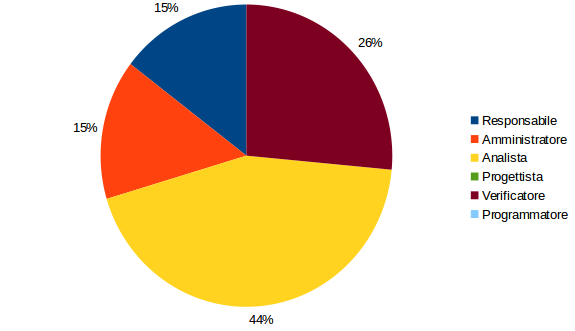
\includegraphics{img_peconomico/oreAnalisi.png}}
	\caption{Ore per ruoli, fase di Analisi di dettaglio}
\end{figure}
\begin{figure}[H]
	\centering
	\scalebox{0.6}{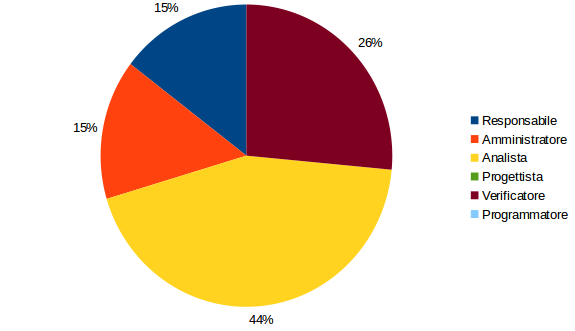
\includegraphics{img_peconomico/oreAnalisi.png}}
	\caption{Costi per ruolo, fase di Analisi di dettaglio}
\end{figure}

\subsection{Progettazione Architetturale}
Nella fase di \textbf{Progettazione Architetturale} le ore sono suddivise nel modo seguente:
\begin{table}[H]
	\centering
	\begin{tabular}{|c|c|c|}
		\hline
		\textbf{Ruolo} &
		\textbf{Ore} &
		\textbf{Costo} \\
		\hline
		Responsabile & 8 & 240\\
		\hline
		Amministratore & 0 & 0\\
		\hline
		Analista & 0 & 0\\
		\hline
		Progettista & 125 & 2750 \\
		\hline
		Programmatore & 0 & 0 \\
		\hline
		Verificatore & 60 & 900\\
		\hline
		\textbf{Totale} & \textbf{193} & \textbf{3890} \\
		\hline
	\end{tabular}
	\caption{Costo per ruolo, fase di Progettazione Architetturale}
\end{table}

I seguenti grafici mostrano visivamente come abbiano influiranno i ruoli per ore e costi nella fase di \textbf{Progettazione Architetturale}.
\begin{figure}[H]
	\centering
	\scalebox{0.6}{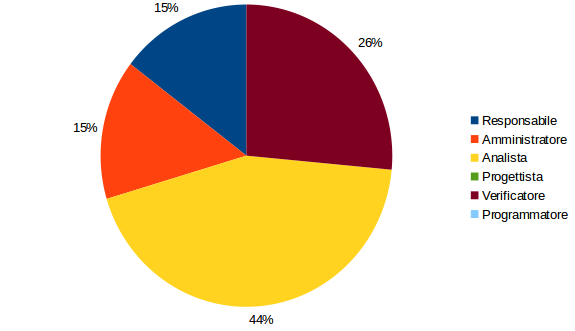
\includegraphics{img_peconomico/oreAnalisi.png}}
	\caption{Ore per ruoli, fase di Progettazione Architetturale}
\end{figure}
\begin{figure}[H]
	\centering
	\scalebox{0.6}{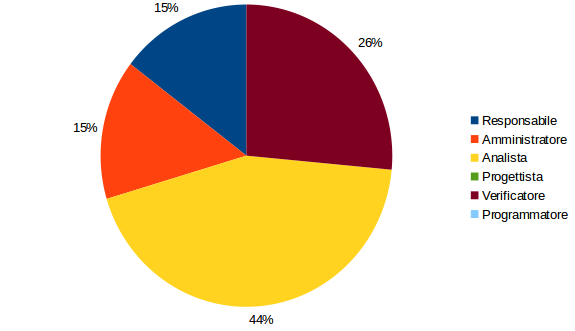
\includegraphics{img_peconomico/oreAnalisi.png}}
	\caption{Costi per ruolo, fase di Progettazione Architetturale}
\end{figure}

\subsection{Progettazione di dettaglio}
Nella fase di \textbf{Progettazione di dettaglio} le ore sono suddivise nel modo seguente:
\begin{table}[H]
	\centering
	\begin{tabular}{|c|c|c|}
		\hline
		\textbf{Ruolo} &
		\textbf{Ore} &
		\textbf{Costo} \\
		\hline
		Responsabile & 8 & 240 \\
		\hline
		Amministratore & 7 & 140 \\
		\hline
		Analista & 0 & 0\\
		\hline
		Progettista & 96 & 2112 \\
		\hline
		Programmatore & 0 & 0 \\
		\hline
		Verificatore & 35 & 525 \\
		\hline
		\textbf{Totale} & \textbf{146} & \textbf{3017} \\
		\hline
	\end{tabular}
	\caption{Costo per ruolo, fase di Progettazione di dettaglio}
\end{table}

I seguenti grafici mostrano visivamente come abbiano influiranno i ruoli per ore e costi nella fase di \textbf{Progettazione di dettaglio}.
\begin{figure}[H]
	\centering
	\scalebox{0.6}{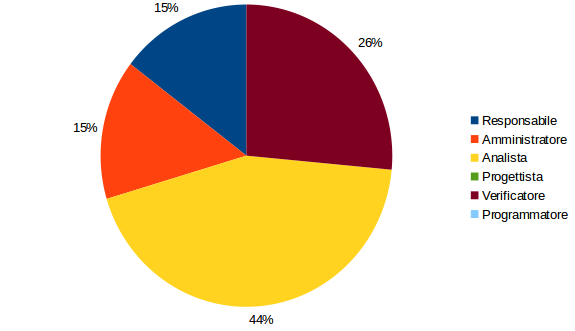
\includegraphics{img_peconomico/oreAnalisi.png}}
	\caption{Ore per ruoli, fase di Progettazione di dettaglio}
\end{figure}
\begin{figure}[H]
	\centering
	\scalebox{0.6}{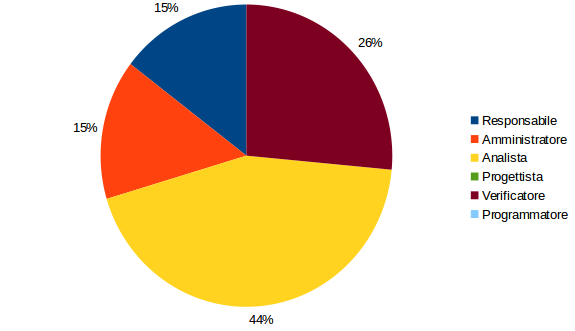
\includegraphics{img_peconomico/oreAnalisi.png}}
	\caption{Costi per ruolo, fase di Progettazione di dettaglio}
\end{figure}

\subsection{Codifica}
Nella fase di \textbf{Codifica} le ore sono suddivise nel modo seguente:
\begin{table}[H]
	\centering
	\begin{tabular}{|c|c|c|}
		\hline
		\textbf{Ruolo} &
		\textbf{Ore} &
		\textbf{Costo} \\
		\hline
		Responsabile & 10 & 300 \\
		\hline
		Amministratore & 4 & 80 \\
		\hline
		Analista & 0 & 0\\
		\hline
		Progettista & 15 & 330 \\
		\hline
		Programmatore & 141 & 2115 \\
		\hline
		Verificatore & 50 & 750 \\
		\hline
		\textbf{Totale} & \textbf{220} & \textbf{3575} \\
		\hline
	\end{tabular}
	\caption{Costo per ruolo, fase di Codifica}
\end{table}

I seguenti grafici mostrano visivamente come abbiano influiranno i ruoli per ore e costi nella fase di \textbf{Codifica}.
\begin{figure}[H]
	\centering
	\scalebox{0.6}{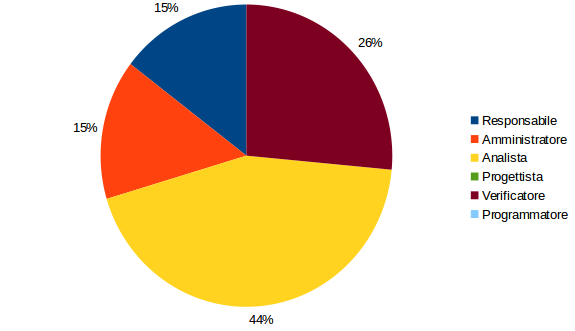
\includegraphics{img_peconomico/oreAnalisi.png}}
	\caption{Ore per ruoli, fase di Codifica}
\end{figure}
\begin{figure}[H]
	\centering
	\scalebox{0.6}{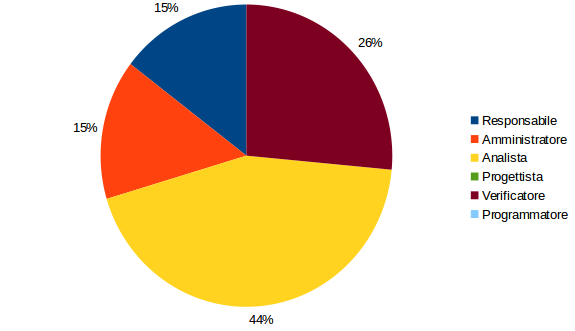
\includegraphics{img_peconomico/oreAnalisi.png}}
	\caption{Costi per ruolo, fase di Codifica}
\end{figure}

\subsection{Verifica e Validazione}
Nella fase di \textbf{Verifica e Validazione} le ore sono suddivise nel modo seguente:
\begin{table}[H]
	\centering
	\begin{tabular}{|c|c|c|}
		\hline
		\textbf{Ruolo} &
		\textbf{Ore} &
		\textbf{Costo} \\
		\hline
		Responsabile & 5 & 150\\
		\hline
		Amministratore & 0 & 0\\
		\hline
		Analista & 0 & 0\\
		\hline
		Progettista & 13 & 286 \\
		\hline
		Programmatore & 0 & 0 \\
		\hline
		Verificatore & 81 & 1215\\
		\hline
		\textbf{Totale} & \textbf{99} & \textbf{1651} \\
		\hline
	\end{tabular}
	\caption{Costo per ruolo, fase di Verifica e Validazione}
\end{table}

I seguenti grafici mostrano visivamente come abbiano influiranno i ruoli per ore e costi nella fase di \textbf{Verifica e Validazione}.
\begin{figure}[H]
	\centering
	\scalebox{0.6}{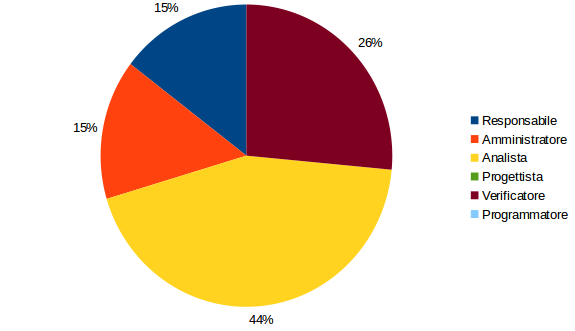
\includegraphics{img_peconomico/oreAnalisi.png}}
	\caption{Ore per ruolo, fase di Verifica e Validazione}
\end{figure}
\begin{figure}[H]
	\centering
	\scalebox{0.6}{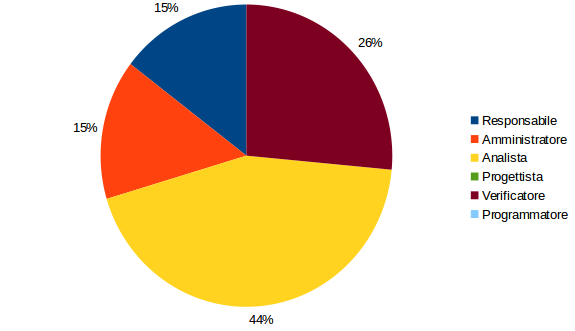
\includegraphics{img_peconomico/oreAnalisi.png}}
	\caption{Costi per ruolo, fase di Verifica e Validazione}
\end{figure}

\subsection{Totale}
\subsubsection{Ore totali con investimento}
Le ore complessive previste per ogni ruolo sono ripostate nella tabella sottsatante.
\begin{table}[H]
	\centering
	\begin{tabular}{|c|c|c|}
		\hline
		\textbf{Ruolo} &
		\textbf{Ore} &
		\textbf{Costo} \\
		\hline
		Responsabile & 67 & 2010\\
		\hline
		Amministratore & 40 & 800\\
		\hline
		Analista & 107 & 2675\\
		\hline
		Progettista & 431 & 9482 \\
		\hline
		Programmatore & 141 & 2115 \\
		\hline
		Verificatore & 271 & 4065\\
		\hline
		\textbf{Totale} & \textbf{1057} & \textbf{21147} \\
		\hline
	\end{tabular}
	\caption{Costo totale per ruolo}
\end{table}
I seguenti grafici mostrano visivamente come abbiano influiranno i ruoli per ore e costi nel progetto.
\begin{figure}[H]
	\centering
	\scalebox{0.6}{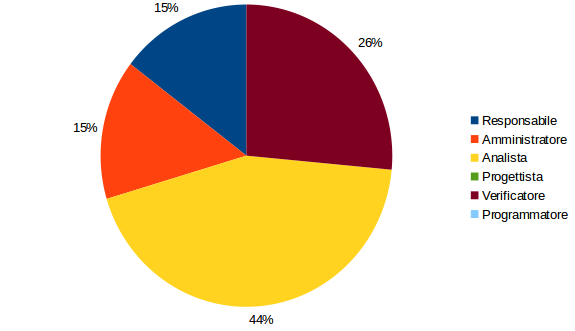
\includegraphics{img_peconomico/oreAnalisi.png}}
	\caption{Ore totali per ruolo}
\end{figure}
\begin{figure}[H]
	\centering
	\scalebox{0.6}{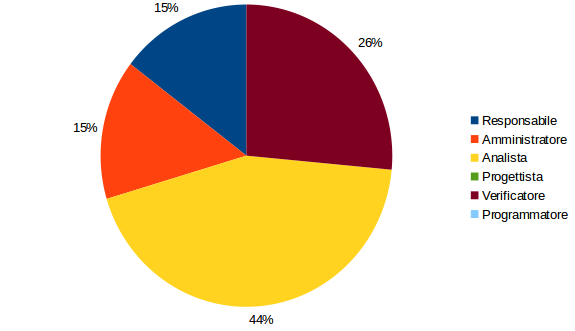
\includegraphics{img_peconomico/oreAnalisi.png}}
	\caption{Costi totali per ruolo}
\end{figure}

\subsubsection{Ore rendicontate}
Le ore complessive rendicontate per ogni ruolo sono ripostate nella tabella sottsatante.
\begin{table}[H]
	\centering
	\begin{tabular}{|c|c|c|}
		\hline
		\textbf{Ruolo} &
		\textbf{Ore} &
		\textbf{Costo} \\
		\hline
		Responsabile & 21 & 630\\
		\hline
		Amministratore & 21.5 & 430\\
		\hline
		Analista & 63 & 1575\\
		\hline
		Progettista & 0 & 0 \\
		\hline
		Programmatore & 0 & 0 \\
		\hline
		Verificatore & 38 & 570\\
		\hline
		\textbf{Totale} & \textbf{143.5} & \textbf{3205} \\
		\hline
	\end{tabular}
	\caption{Costo totale per ruolo}
\end{table}
I seguenti grafici mostrano visivamente come abbiano influiranno i ruoli per ore e costi nel progetto.
\begin{figure}[H]
	\centering
	\scalebox{0.6}{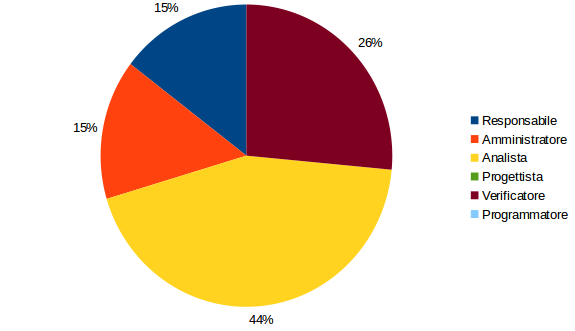
\includegraphics{img_peconomico/oreAnalisi.png}}
	\caption{Ore totali per ruolo}
\end{figure}
\begin{figure}[H]
	\centering
	\scalebox{0.6}{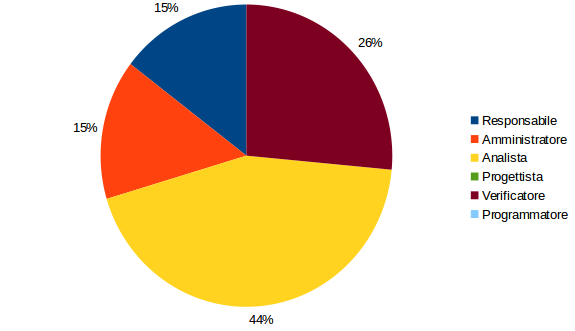
\includegraphics{img_peconomico/oreAnalisi.png}}
	\caption{Costi totali per ruolo}
\end{figure}





